

%% AAPT Physics Bowl Exams Questions
%%----------------------------------------


%% This section has XX problems


%% PhysicsBowl 2015
%%----------------------------------------
\element{aapt}{ %% Bowl-D1
\begin{question}{bowl-2015-q08}
    A negatively charged balloon remains at rest when placed on a vertical wall.
    Which one of the following terms is most closely associated with the
        electrical phenomenon allowing the balloon to remain on the wall?
    \begin{multicols}{2}
    \begin{choices}
        \wrongchoice{Radiation}
        \wrongchoice{Grounding}
        \wrongchoice{Reduction}
        \wrongchoice{Current}
      \correctchoice{Polarization}
    \end{choices}
    \end{multicols}
\end{question}
}

\element{aapt}{ %% Bowl-D1
\begin{question}{bowl-2015-q45}
    A \SI{6.00}{\micro\farad} parallel-plate capacitor is disconnected
        from a \SI{12}{\volt} battery after being fully charged.
    A person now carefully inserts a dielectric material of constant
        $\kappa=2$ so that it fills one-half of the space between the plates as shown.
    \begin{center}
    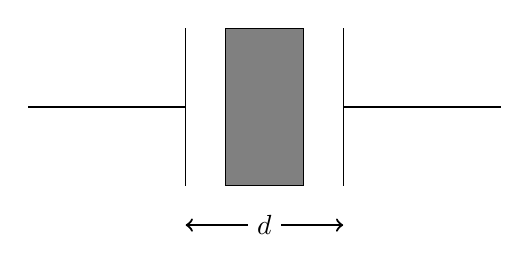
\begin{tikzpicture}
        %% Left Capacitor Plate
        \draw (-1,0) -- (-1,2);
        \draw (-3,1) -- (-1,1);
        %% Right Capacitor Plate
        \draw (+1,0) -- (+1,2);
        \draw (+3,1) -- (+1,1);
        %% Thickness
        \draw[thick,<->] (-1,-0.5) -- (+1,-0.5)
            node[pos=0.5,anchor=center,fill=white] {$d$};
        %% Dielectric
        \draw[fill=white!50!black] (-0.5,0) rectangle (+0.5,2);
    \end{tikzpicture}
    \end{center}
    How much work was done by the person while inserting the dielectric?
    \begin{multicols}{3}
    \begin{choices}
        \wrongchoice{\SI{-81}{\micro\joule}}
      \correctchoice{\SI{-108}{\micro\joule}}
        \wrongchoice{\SI{-144}{\micro\joule}}
        \wrongchoice{\SI{-216}{\micro\joule}}
        \wrongchoice{\SI{-288}{\micro\joule}}
    \end{choices}
    \end{multicols}
\end{question}
}

\element{aapt}{ %% Bowl-D1
\begin{question}{bowl-2015-q48}
    Two concentric charged conducting shells are in free space.
    The outer shell has inner radius $2a$ and outer radius $3a$.
    The inner shell has radius $a$.
    \begin{center}
    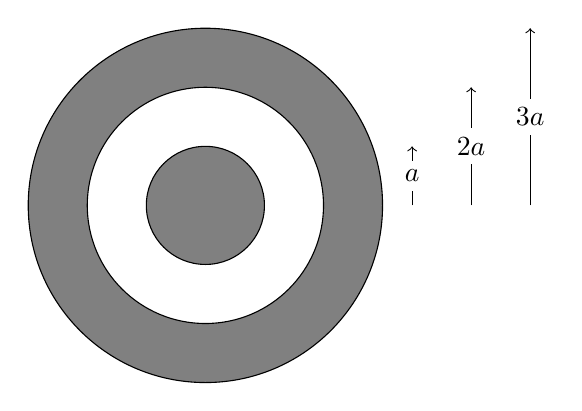
\begin{tikzpicture}[scale=0.75]
        \draw[fill=white!50!black] (0,0) circle (3.0cm);
        \draw[fill=white]          (0,0) circle (2.0cm);
        \draw[fill=white!50!black] (0,0) circle (1.0cm);
        \draw[->] (3.5,0) -- ++ (90:1cm) node[fill=white,anchor=center,pos=0.5] {$a$};
        \draw[->] (4.5,0) -- ++ (90:2cm) node[fill=white,anchor=center,pos=0.5] {$2a$};
        \draw[->] (5.5,0) -- ++ (90:3cm) node[fill=white,anchor=center,pos=0.5] {$3a$};
    \end{tikzpicture}
    \end{center}
    It is known that the electric potential at $r=3a$ is $V_{3a}= \frac{kQ}{3a}$.
    If the electric potential $V_{a}$ at $r=a$ is \SI{0}{\volt},
        what is the charge on the inner spherical shell, $Q_{in}$?
    \begin{multicols}{2}
    \begin{choices}
        \wrongchoice{$Q_{in}= -\frac{3}{2} Q$}
      \correctchoice{$Q_{in}= -\frac{2}{3} Q$}
        \wrongchoice{$Q_{in}= -\frac{1}{3} Q$}
        \wrongchoice{$Q_{in}= - 2Q$}
        \wrongchoice{$Q_{in}= -\frac{1}{2} Q$}
    \end{choices}
    \end{multicols}
\end{question}
}


%% PhysicsBowl 2014
%%----------------------------------------
\element{aapt}{ %% Bowl-D1
\begin{question}{bowl-2014-q10}
    Two charges, $-Q$ and $+Q$, are fixed in place on the $x$-axis,
        each a distance $a$ from the origin as shown.
    \begin{center}
    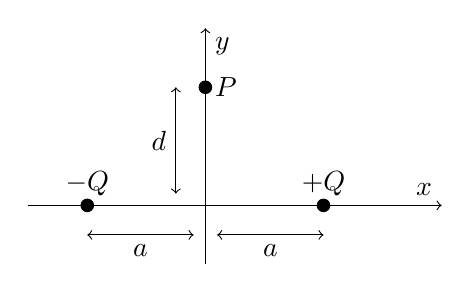
\begin{tikzpicture}[scale=1.5]
        %% Axes
        \draw[->] (-1.5,0) -- (2,0) node[pos=1.0,anchor=south east] {$x$};
        \draw[->] (0,-0.5) -- (0,1.5) node[pos=1.0,anchor=north west] {$y$};
        %% Location labels
        \draw[fill] (-1,0) circle (1.5pt) node[anchor=south] {$-Q$};
        \draw[fill] (+1,0) circle (1.5pt) node[anchor=south] {$+Q$};
        \draw[fill] (0,+1) circle (1.5pt) node[anchor=west] {$P$};
        %% Distance labels
        \draw[<->] (-1,-0.25) -- (-0.1,-0.25) node[pos=0.5,anchor=north] {$a$};
        \draw[<->] (+1,-0.25) -- (0.1,-0.25) node[pos=0.5,anchor=north] {$a$};
        \draw[<->] (-0.25,1) -- (-0.25,0.1) node[pos=0.5,anchor=east] {$d$};
    \end{tikzpicture}
    \end{center}
    At the point labeled $P$, a distance $d$ along the $y$-axis from the origin,
        what is the direction of the electric field from the given charges?
    \begin{choices}
        \wrongchoice{Up the plan of the page}
        \wrongchoice{Down the plane of the page}
        \wrongchoice{To the right}
      \correctchoice{To the left}
        \wrongchoice{There is no electric field}
    \end{choices}
\end{question}
}

\element{aapt}{ %% Bowl-D1
\begin{question}{bowl-2014-q47}
    An air-filled parallel plate capacitor of capacitance $C$ is fully charged after being connected to a battery of voltage $V$.
    The battery then is disconnected and an insulating dielectric slave of constant $\kappa$ is inserted between the capacitor's plates,
        fully filling the region.
    What is the voltage between the plates once equilibrium is established with the dielectric in place?
    \begin{multicols}{3}
    \begin{choices}
        \wrongchoice{$\kappa^2V$}
        \wrongchoice{$\kappa V$}
        \wrongchoice{$V$}
      \correctchoice{$\dfrac{V}{\kappa}$}
        \wrongchoice{$\dfrac{V}{\kappa^2}$}
    \end{choices}
    \end{multicols}
\end{question}
}


%% PhysicsBowl 2013
%%----------------------------------------
\element{aapt}{ %% Bowl-D1
\begin{question}{bowl-2013-q07}
    Two identical particles are fixed in place a distance of \SI{0.50}{\meter} apart.
    The electric force that one particle exerts on the other has a magnitude of \SI{3.00}{\newton}.
    Which one of the following choices best represents the magnitude of each particle's charge?
    \begin{multicols}{2}
    \begin{choices}
        \wrongchoice{\SI{4.17e-11}{\coulomb}}
        \wrongchoice{\SI{8.33e-11}{\coulomb}}
        \wrongchoice{\SI{1.67e-10}{\coulomb}}
      \correctchoice{\SI{9.13e-6}{\coulomb}}
        \wrongchoice{\SI{1.29e-5}{\coulomb}}
    \end{choices}
    \end{multicols}
\end{question}
}

\element{aapt}{ %% Bowl-D1
\begin{question}{bowl-2013-q29}
    Two electrons enter a region between charged capacitor plates with equal speed $v$.
    \begin{center}
    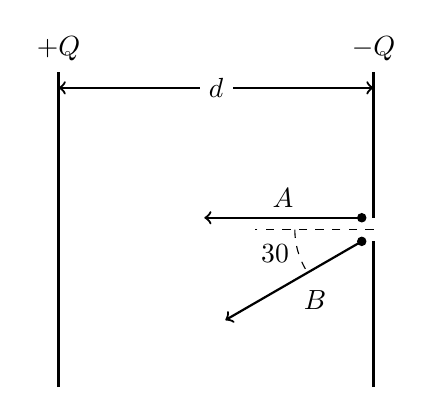
\begin{tikzpicture}
        %% Plates
        \draw[very thick] (-2,-2) -- (-2,+2) node[anchor=south] {$+Q$};
        \draw[very thick] (+2,-2) -- (+2,+2) node[anchor=south] {$-Q$};
        %% Gap
        \fill[white] (+1.9,-0.15) rectangle (+2.1,+0.15);
        %% Distance
        \draw[thick,<->] (-2,1.8) -- (+2,1.8) node[pos=0.5,anchor=center,fill=white] {$d$};
        %% Two electrons A and B
        \coordinate (A) at (1.85,+0.15);
        \coordinate (B) at (1.85,-0.15);
        \draw[fill] (A) circle (1.5pt);
        \draw[fill] (B) circle (1.5pt);
        \draw[thick,->] (A) -- ++ (180:2.0cm) node[pos=0.5,anchor=south] {$A$};
        \draw[thick,->] (B) -- ++ (210:2.0cm) node[pos=0.5,anchor=north west] {$B$};
        %% 30 degrees
        \draw[dashed] (2,0) -- ++ (180:1.5cm);
        \draw[dashed] (2,0) ++ (180:1.0cm) arc (180:210:1.0) node[pos=0.6,anchor=east] {\ang{30}};
    \end{tikzpicture}
    \end{center}
    Electron $A$ is directed horizontally to the left while electron $B$ is directed at \ang{30} below the horizontal.
    Each electron makes it to the left-hand plate.
    Which one of the following choices best compares the speeds of the charges $(v_A,v_B)$ upon arrival at the left plate?
    Consider only the electrons $A$ and $B$'s interactions with the constant electric field between the plates, ignoring any relativistic effects.
    \begin{choices}
        \wrongchoice{$v_A > v_B$}
      \correctchoice{$v_A = v_B$}
        \wrongchoice{$v_A < v_B$}
        \wrongchoice{The answer depends on the size of the plate separation $d$.}
        \wrongchoice{The answer depends on the magnitude of the charge, $Q$, on each plate.}
    \end{choices}
\end{question}
}


%% PhysicsBowl 2012
%%----------------------------------------
\element{aapt}{ %% Bowl-D1
\begin{question}{bowl-2012-q13}
    Approximately how many electrons must be removed from
        an electrically neutral object to give it a net
        charge of $Q=\SI[retain-explicit-plus]{+1.00}{\coulomb}$?
    \begin{multicols}{2}
    \begin{choices}
        \wrongchoice{\num{1.60e-19}}
        \wrongchoice{\num{1}}
      \correctchoice{\num{6.25e18}}
        \wrongchoice{\num{6.02e23}}
        \wrongchoice{\num{1.1e30}}
    \end{choices}
    \end{multicols}
\end{question}
}

\element{aapt}{ %% Bowl-D1
\begin{question}{bowl-2012-q31}
    Three particles with charges $Q$, $Q$, and $Q_2$ are initially at rest very (infinitely) far apart from one another.
    The particles are moved to the locations shown in the figure where they are fixed in place.
    The particles on the left and right have charge $Q$ and are separated by a distance $R$.
    The particle with charge $Q_2$ is located at the midpoint directly between the other charged particles.
    \begin{center}
    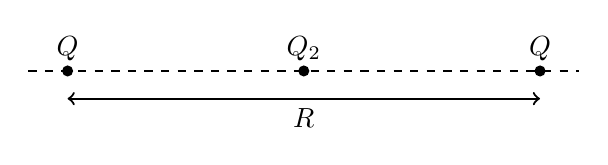
\begin{tikzpicture}
        %% Axis
        \draw[dashed] (-3.5,0) -- (3.5,0);
        %% Charges
        \fill (-3,0) circle (2pt) node[anchor=south] {$Q$};
        \fill ( 0,0) circle (2pt) node[anchor=south] {$Q_2$};
        \fill (+3,0) circle (2pt) node[anchor=south] {$Q$};
        %% Radius label
        \draw[thick,<->] (-3,-1em) -- (+3,-1em) node[pos=0.5,anchor=north] {$R$};
    \end{tikzpicture}
    \end{center}
    The total work required to configure this three-particle arrangement is zero joules.
    Ignore any self-energies for the particles.
    What is the value of the charge $Q_2$?
    %\begin{multicols}{2}
    \begin{choices}
      \correctchoice{$\dfrac{-1}{4}Q$}
        \wrongchoice{$\dfrac{-\sqrt{2}}{4}Q$}
        \wrongchoice{$\dfrac{-1}{2}Q$}
        \wrongchoice{$\dfrac{-1}{8}Q$}
        \wrongchoice{It is not possible to accomplish what is required.}
    \end{choices}
    %\end{multicols}
\end{question}
}


%% PhysicsBowl 2011
%%----------------------------------------
\element{aapt}{ %% Bowl-D1
\begin{question}{bowl-2011-q05}
    A positively charged rod is brought near a metal electroscope that is initially uncharged.
    As shown in the figure, the rod does not touch the electroscope.
    \begin{center}
    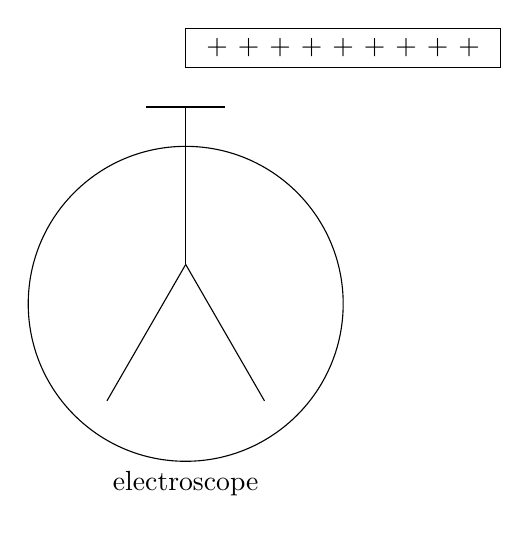
\begin{tikzpicture}
        %% charges rod
        \draw (0,0) rectangle (4,0.5);
        \foreach \x in {4,8,...,36} \node[anchor=center] at (\x mm,0.25) {$+$};
        %% electroscope
        \draw[thick] (-0.5,-0.5) -- (0.5,-0.5);
        \draw (0,-0.5) -- (0,-2.5);
        \draw (0,-2.5) -- ++(300:2);
        \draw (0,-2.5) -- ++(240:2);
        \draw (0,-3) circle (2cm);
        \node[anchor=north] at (0,-5) {electroscope};
    \end{tikzpicture}
    \end{center}
    There is no charge transfer between the electroscope and rod,
        but the leaves of the electroscope move apart from each other when the rod is brought near the top of the electroscope.
    Which one of the following choices is the best explanation for this phenomenon?
    \begin{choices}
        \wrongchoice{Protons are repelled by the rod into the leaves of the electroscope.}
      \correctchoice{Electrons are attracted out of the leaves of the electroscope toward the rod.}
        \wrongchoice{Protons are repelled into the leaves of the electroscope and electrons are attracted out of the leaves of the electroscope.}
        \wrongchoice{Positively charged electrons are repelled by the rod into the leaves of the electroscope.}
        \wrongchoice{Positively charged electrons are repelled into the leaves of the electroscope and regular electrons are attracted out of the leaves of the electroscope.}
    \end{choices}
\end{question}
}

\element{aapt}{ %% Bowl-D1
\begin{question}{bowl-2011-q16}
    Which one of the following is \emph{not} a vector quantity?
    \begin{choices}
        \wrongchoice{Linear momentum}
        \wrongchoice{Electric field}
        \wrongchoice{Average velocity}
        \wrongchoice{Instantaneous acceleration}
      \correctchoice{Kinetic energy}
    \end{choices}
\end{question}
}

\element{aapt}{ %% Bowl-D1
\begin{question}{bowl-2011-q42}
    A parallel-plate capacitor of capacitance $C$ has an insulating dielectric material of constant $\kappa$ filling the entire region between the plates.
    This capacitance is connect to a battery of voltage $V$ and is fully charged before the battery is disconnected.
    The capacitor stores energy $U$.
    Using insulating gloves, a person now removes the dielectric from the capacitor.
    After equilibrium is established following the removal of the dielectric,
        which one of the following choices represents the energy stored by the capacitor in terms of $U$?
    \begin{multicols}{3}
    \begin{choices}
        \wrongchoice{$\kappa^2 U$}
      \correctchoice{$\kappa U$}
        \wrongchoice{$U$}
        \wrongchoice{$\dfrac{U}{\kappa}$}
        \wrongchoice{$\dfrac{U}{\kappa^2}$}
    \end{choices}
    \end{multicols}
\end{question}
}

\element{aapt}{ %% Bowl-D1
\begin{question}{bowl-2011-q46}
    A hollow conducting sphere in static equilibrium is isolated in deep space with a net excess charge $+Q$ on it.
    \begin{center}
    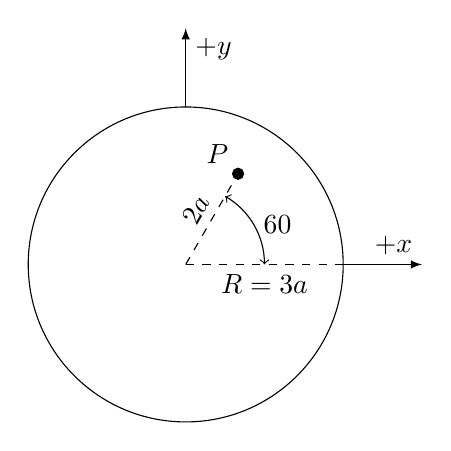
\begin{tikzpicture}
        %% cyclinder
        \draw (0,0) circle (2);
        %% axes
        \draw [dashed] (0,0) -- (2,0) node[pos=0.5,anchor=north] {$R=3a$};
        \draw[-latex] (2,0) -- (3,0) node[anchor=south east] {$+x$};
        \draw[-latex] (0,2) -- (0,3) node[anchor=north west] {$+y$};
        %% Point P
        \draw[dashed] (0,0) -- (60:1.33) node[pos=0.5,anchor=south,rotate=60] {$2a$};
        \draw[fill] (60:1.33) circle (2pt) node[anchor=south east] {$P$};
        \draw[<->] (1,0) arc (0:60:1) node[pos=0.5,anchor=west] {\ang{60}};
    \end{tikzpicture}
    \end{center}
    What is the electric potential (assuming $V\left(r\rightarrow\infty\right)=0$)
        at the position labeled $P$ shown in the interior of the figure?
    The sphere has radius $R=3a$ and the point of interest is at a location $r=2a$ from the center of the sphere at an angle of \ang{60} with respect to the $x$-axis.
    \begin{multicols}{3}
    \begin{choices}
        \wrongchoice{zero}
        \wrongchoice{$\dfrac{kQ}{2a}$}
      \correctchoice{$\dfrac{kQ}{3a}$}
        \wrongchoice{$\dfrac{kQ}{4a}$}
        \wrongchoice{$\dfrac{\sqrt{3}kQ}{4a}$}
    \end{choices}
    \end{multicols}
\end{question}
}


%% PhysicsBowl 2010
%%----------------------------------------
\element{aapt}{ %% Bowl-D1
\begin{question}{bowl-2010-q12}
    A scientist sets up an experiment with a proton of charge $+Q$ and mass $M$ being placed near a helium  nucleus (2 protons and 2 neutrons) of charge $+2Q$ and mass $4M$.
    The objects are each released from rest and begin to move.
    From the scientist's point of view, which choice best describes the object that experiences the greatest magnitude of electric force from the other and which object experiences the greatest magnitude of acceleration?
    Ignore gravity?
    \begin{center}
    \begin{tabu}{cX[c]X[c]}
        \toprule
        \makebox[1.5em][c]{\textnumero}
            & Largest magnitude of force & Largest magnitude of acceleration \\
        \bottomrule
    \end{tabu}
    \end{center}
    \begin{choices}
        \wrongchoice{\begin{tabu}{X[c]X[c]} The helium nucleus & The helium nucleus \\ \end{tabu}}
        \wrongchoice{\begin{tabu}{X[c]X[c]} The helium nucleus & The proton \\ \end{tabu}}
        \wrongchoice{\begin{tabu}{X[c]X[c]} The proton          & The accelerations are equal \\ \end{tabu}}
        \wrongchoice{\begin{tabu}{X[c]X[c]} The forces are equal & The accelerations are equal \\ \end{tabu}}
      \correctchoice{\begin{tabu}{X[c]X[c]} The forces are equal & The proton \\ \end{tabu}}
    \end{choices}
\end{question}
}

\element{aapt}{ %% Bowl-D1
\begin{question}{bowl-2010-q36}
    In terms of the seven fundamental SI units in the MKS system,
        the unit for capacitance is written as which of the following?
    \begin{multicols}{3}
    \begin{choices}
        \wrongchoice{$\dfrac{\si{\ampere\squared}}{\si{\kilo\gram\meter\squared}}$}
        \wrongchoice{$\dfrac{\si{\ampere\second}}{\si{\kilo\gram\meter\squared}}$}
        \wrongchoice{$\dfrac{\si{\ampere\second\squared}}{\si{\kilo\gram\meter}}$}
        \wrongchoice{$\dfrac{\si{\ampere\squared\second\cubed}}{\si{\kilo\gram\meter\squared}}$}
      \correctchoice{$\dfrac{\si{\ampere\squared\second\tothefourth}}{\si{\kilo\gram\meter\squared}}$}
    \end{choices}
    \end{multicols}
\end{question}
}

\element{aapt}{ %% Bowl-D1
\begin{question}{bowl-2010-q37}
    A positively charged particle is moved in a straight line
        to the right from position $x=\SI{-4.0}{\meter}$ to
        position $x=\SI{-2.0}{\meter}$ by an external agent.
    The electric potential at these positions in space are
        $V(x=\SI{-4}{\meter})=\SI{-4.0}{\volt}$ and
        $V(x=\SI{-2}{\meter})=\SI{-2.0}{\volt}$.
    Which statement is true about the work done by the
        external agent moving the charge between these
        positions and the electric field component parallel
        to the direction of motion that the moving charged
        particle experiences?
    Assume the particle is moved at constant speed.
    \begin{choices}
        \wrongchoice{The external agent does no work since the speed was constant.}
        \wrongchoice{The external agent does negative work and the electric field is directed to the right.}
        \wrongchoice{The external agent does positive work and the electric field is directed to the right.}
        \wrongchoice{The external agent does negative work and the electric field is directed to the left.}
      \correctchoice{The external agent does positive work and the electric field is directed to the left.}
    \end{choices}
\end{question}
}


%% PhysicsBowl 2009
%%----------------------------------------
\element{aapt}{ %% Bowl-D1
\begin{question}{bowl-2009-q23}
    A personal rubs a neutral comb through their hair and the
        comb becomes negatively charged.
    Which of the following is the best explanation for this phenomenon?
    \begin{choices}
        \wrongchoice{The hair gains protons from the comb.}
        \wrongchoice{The hair gains protons from the comb while giving electrons to the comb.}
      \correctchoice{The hair loses electrons to the comb.}
        \wrongchoice{The comb loses protons to the person's hand holding the comb.}
        \wrongchoice{The comb loses protons to the person's hand while also gaining electrons from the hair.}
    \end{choices}
\end{question}
}


%% PhysicsBowl 2008
%%----------------------------------------
\element{aapt}{ %% Bowl-D1
\begin{question}{bowl-2008-q06}
    A positive point charge exerts a force of magnitude $F$ on a negative point charge placed a distance $x$ away.
    If the distance between the two point charges is halved,
        what is the magnitude of the new force that the positive point charge exerts on the negative point charge?
    \begin{multicols}{3}
    \begin{choices}
      \correctchoice{$4F$}
        \wrongchoice{$2F$}
        \wrongchoice{$F$}
        \wrongchoice{$\frac{F}{2}$}
        \wrongchoice{$\frac{F}{4}$}
    \end{choices}
    \end{multicols}
\end{question}
}

\newcommand{\BowlTwentyZeroEightQThirtyThree}{
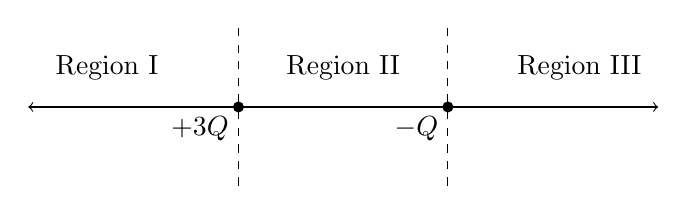
\begin{tikzpicture}
    %% axis
    \draw[<->] (-4,0) -- (4,0);
    %% charges
    \fill (-1.33,0) circle (2pt) node[anchor=north east] {$+3Q$};
    \fill (+1.33,0) circle (2pt) node[anchor=north east] {$-Q$};
    %% dashed
    \draw[dashed] (-1.33,-1) -- (-1.33,+1);
    \draw[dashed] (+1.33,-1) -- (+1.33,+1);
    %% labels
    \node[anchor=center] at (-3,0.5) {Region I};
    \node[anchor=center] at (0,0.5) {Region II};
    \node[anchor=center] at (+3,0.5) {Region III};
\end{tikzpicture}
}

\element{aapt}{ %% Bowl-D1
\begin{question}{bowl-2008-q33}
    Two point charges are fixed on the $x$-axis in otherwise empty space as shown below.
    \begin{center}
        \BowlTwentyZeroEightQThirtyThree
    \end{center}
    %% start question
    In which Region(s) is there a place on the $x$-axis (aside from infinity) at which the electric potential is equal to zero?
    \begin{choices}
        \wrongchoice{Only in Region II}
        \wrongchoice{Only in Region III}
        \wrongchoice{In both Regions I and II}
        \wrongchoice{In both Regions I and III}
      \correctchoice{In both Regions II and III}
    \end{choices}
\end{question}
}

\element{aapt}{ %% Bowl-D1
\begin{question}{bowl-2008-q34}
    Two point charges are fixed on the $x$-axis in otherwise empty space as shown below.
    \begin{center}
        \BowlTwentyZeroEightQThirtyThree
    \end{center}
    %% start question
    In which Region(s) is there a place on the $x$-axis (aside from infinity) at which the electric field is equal to zero?
    \begin{choices}
        \wrongchoice{Only in Region II}
      \correctchoice{Only in Region III}
        \wrongchoice{In both Regions I and II}
        \wrongchoice{In both Regions I and III}
        \wrongchoice{In both Regions II and III}
    \end{choices}
\end{question}
}


%% PhysicsBowl 2007
%%----------------------------------------
\element{aapt}{ %% Bowl-D1
\begin{question}{bowl-2007-q25}
    If two protons are spaced by a distance $R$,
        what is the ratio of the gravitational force that one proton exerts on the other to the electric force that one proton exerts on the other?
    That is:
    \begin{equation*}
        \frac{F_{gravity}}{F_{electric}} =
    \end{equation*}
    \begin{multicols}{3}
    \begin{choices}
        \wrongchoice{$\approx\num{e-8}$}
        \wrongchoice{$\approx\num{e-16}$}
        \wrongchoice{$\approx\num{e-20}$}
      \correctchoice{$\approx\num{e-36}$}
        \wrongchoice{$\approx\num{e-43}$}
    \end{choices}
    \end{multicols}
\end{question}
}

\element{aapt}{ %% Bowl-D1
\begin{question}{bowl-2007-q28}
    Which statement about a system of point charges that are fixed in space is necessarily true?
    \begin{choices}
      \correctchoice{If the potential energy of the system is negative,
            net positive work by an external agent is required to take the charges in the system back to infinity.}
        \wrongchoice{If the potential energy of the system is positive,
            net positive work is required to bring any new charge not part of the system in from infinity to its final resting location.}
        \wrongchoice{If the potential energy of the system is zero,
            no negative charges are in the configuration}
        \wrongchoice{If the potential energy of the system is negative,
            net positive work by an external agent was required to assemble the system of charges.}
        \wrongchoice{If the potential energy of the system is zero,
            then there is no electric force anywhere in space on any other charged particle not part of the system.}
    \end{choices}
\end{question}
}


%% PhysicsBowl 2005
%%----------------------------------------
\element{aapt}{ %% Bowl-D1
\begin{question}{bowl-2005-q45}
    A spherical conducting shell has a net charge $+Q$ placed on it.
    Which of the following is the correct relationship for the electric potential at the points labeled $A$, $B$, and $C$?
    Point $A$ is at the center of the sphere,
        point $B$ is at the surface of the shell, a distance $R$ from point $A$,
        and point $C$ is a distance $R$ from point $B$ outside the sphere.
    \begin{center}
    \begin{tikzpicture}
        %% spherical shell
        \draw (0,0) circle (2);
        %% Points A, B, C
        \fill (0,0) circle (2pt) node[anchor=south] {$A$};
        \fill (2,0) circle (2pt) node[anchor=south west] {$B$};
        \fill (4,0) circle (2pt) node[anchor=south] {$C$};
        %% Radius
        \draw[thick,<->] (0,2.25) -- (2,2.25) node[pos=0.5,anchor=center,fill=white] {$R$};
        \draw[thick,<->] (2,2.25) -- (4,2.25) node[pos=0.5,anchor=center,fill=white] {$R$};
    \end{tikzpicture}
    \end{center}
    As $r$ goes to infinity, $V=0$.
    \begin{choices}
        \wrongchoice{$V_C < V_B < V_A$}
        \wrongchoice{$V_A < V_B < V_C$}
        \wrongchoice{$V_C = V_B = V_A$}
        \wrongchoice{$V_C = V_B < V_A$}
      \correctchoice{$V_C < V_B = V_A$}
    \end{choices}
\end{question}
}


%% PhysicsBowl 2000
%%----------------------------------------
\element{aapt}{ %% Bowl-D1
\begin{question}{bowl-2000-q06}
    How much work would be required to move a \SI{4}{\coulomb} charge
        \SI{6}{\meter} parallel to a \SI{24}{\newton\per\coulomb} electric field?
    \begin{multicols}{3}
    \begin{choices}
        \wrongchoice{\SI{0}{\joule}}
        \wrongchoice{\SI{24}{\joule}}
        \wrongchoice{\SI{96}{\joule}}
        \wrongchoice{\SI{144}{\joule}}
      \correctchoice{\SI{576}{\joule}}
    \end{choices}
    \end{multicols}
\end{question}
}

\element{aapt}{ %% Bowl-D1
\begin{question}{bowl-2000-q17}
    An alpha particle and a proton are placed equal distance between two large charged metal plates as shown.
    \begin{center}
    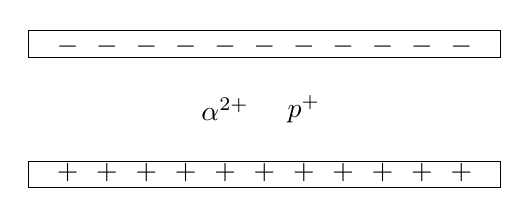
\begin{tikzpicture}
        %% alpha and proton
        \node at (-0.5,0) {$\alpha^{2+}$};
        \node at (+0.5,0) {$p^{+}$};
        %% upper plate
        \draw (-3,0.66) rectangle (+3,1.00);
        \foreach \x in {-25,-20,...,25}
            \node[anchor=center] at (\x mm,0.8) {$-$};
        %% lower plate
        \draw (-3,-0.66) rectangle (+3,-1.00);
        \foreach \x in {-25,-20,...,25}
            \node[anchor=center] at (\x mm,-0.8) {$+$};
    \end{tikzpicture}
    \end{center}
    Which of the following would best describe the motion of the two particles if they were free to move?
    \begin{choices}
        \wrongchoice{The alpha particle will travel upwards with twice the velocity of the proton.}
        \wrongchoice{Both particles will travel upwards with the same velocity.}
        \wrongchoice{The alpha particle will accelerate upwards with twice the acceleration of the proton.}
        \wrongchoice{Both particles will accelerate upwards with the same acceleration.}
      \correctchoice{The alpha particle will accelerate upwards with half the acceleration of the proton.}
    \end{choices}
\end{question}
}

\element{aapt}{ %% Bowl-D1
\begin{questionmult}{bowl-2000-q18}
    Two parallel metal plates carry opposite electrical charges each with a magnitude of $Q$.
    The plates are separated by a distance $d$ and each plate has an area $A$.
    Which of the following would have the effect of reducing the potential difference between the plates?
    \begin{choices}
        \wrongchoice{increasing $Q$}
        \wrongchoice{increasing $d$}
      \correctchoice{increasing $A$}
    \end{choices}
\end{questionmult}
}

\element{aapt}{ %% Bowl-D1
\begin{question}{bowl-1998-q08}
    When two charged point-like objects are separated by a distance $R$,
        the force between them is $F$.
    If the distance between them is quadrupled,
        the force between them is:
    \begin{multicols}{3}
    \begin{choices}
        \wrongchoice{$16 F$}
        \wrongchoice{$4 F$}
        \wrongchoice{$F$}
        \wrongchoice{$\dfrac{F}{4}$}
      \correctchoice{$\dfrac{F}{16}$}
    \end{choices}
    \end{multicols}
\end{question}
}

\element{aapt}{ %% Bowl-D1
\begin{question}{bowl-1998-q30}
    Four positive point charges are arranged as shown in the accompanying diagram.
    \begin{center}
    \begin{tikzpicture}
        %% x and y axis
        \draw (-3,0) -- (3,0);
        \draw (0,-1) -- (0,3);
        %% charges 1,2,3,4
        \fill (0,2) circle (3pt) node[anchor=north west] {1};
        \fill (-2,0) circle (3pt) node[anchor=north west] {2};
        \fill (0,0) circle (3pt) node[anchor=north west] {3};
        \fill (+2,0) circle (3pt) node[anchor=north west] {4};
    \end{tikzpicture}
    \end{center}
    The force between charges 1 and 3 is \SI{6.0}{\newton};
        the force between charges 2 and 3 is \SI{5.0}{\newton};
        and the force between charges 3 and 4 is \SI{3.0}{\newton}.
    The magnitude of the total force on charge 3 is most nearly:
    \begin{multicols}{3}
    \begin{choices}
      \correctchoice{\SI{6.3}{\newton}}
        \wrongchoice{\SI{8.0}{\newton}}
        \wrongchoice{\SI{10}{\newton}}
        \wrongchoice{\SI{11}{\newton}}
        \wrongchoice{\SI{14}{\newton}}
    \end{choices}
    \end{multicols}
\end{question}
}

\element{aapt}{ %% Bowl-D1
\begin{questionmult}{bowl-1998-q37}
    Two isolated parallel plates are separated by a distance $d$.
    They carry opposite charges $Q$ and each has surface area $A$.
    Which of the following would increase the strength of the electric field between the plates?
    \begin{choices}
      \correctchoice{Increasing $Q$}
        \wrongchoice{Increasing $A$}
        \wrongchoice{Increasing $d$}
    \end{choices}
\end{questionmult}
}


%% PhysicsBowl 1997
%%----------------------------------------
\element{aapt}{ %% Bowl-D1
\begin{question}{bowl-1997-q06}
    A charged rod is placed between two insulated conducting spheres as shown.
    The spheres have no net charge.
    \begin{center}
    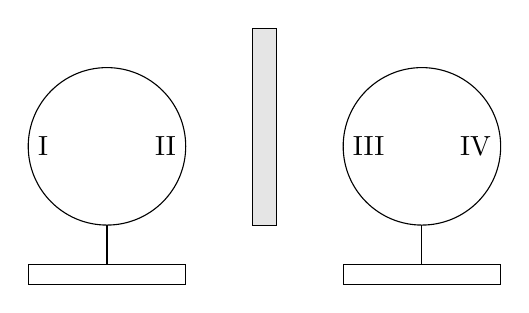
\begin{tikzpicture}
        %% Rod
        \begin{scope}
            \draw[fill=white!90!black] (-1ex,0) rectangle (1ex,2.5);
        \end{scope}
        %% left conducting sphere
        \begin{scope}[xshift=-2cm]
            \draw (0,1) circle (1cm);
            \node[anchor=west] at (-1,1) {I};
            \node[anchor=east] at (+1,1) {II};
            \draw (0,0) -- (0,-0.5);
            \draw (-1,-0.5) rectangle (1,-0.75);
        \end{scope}
        %% right conducting sphere
        \begin{scope}[xshift=+2cm]
            \draw (0,1) circle (1cm);
            \node[anchor=west] at (-1,1) {III};
            \node[anchor=east] at (+1,1) {IV};
            \draw (0,0) -- (0,-0.5);
            \draw (-1,-0.5) rectangle (1,-0.75);
        \end{scope}
    \end{tikzpicture}
    \end{center}
    Region II has the same polarity as Region:
    \begin{multicols}{2}
    \begin{choices}
        \wrongchoice{I only}
      \correctchoice{III only}
        \wrongchoice{IV only}
        \wrongchoice{I \& II only}
        \wrongchoice{I \& IV only}
    \end{choices}
    \end{multicols}
\end{question}
}

\element{aapt}{ %% Bowl-D1
\begin{question}{bowl-1997-q16}
    How much work is required to move \SI{-24}{\micro\coulomb} of charge \SI{4.0}{\meter} parallel to a uniform \SI{6.0}{\newton\per\coulomb} electric field?
    \begin{multicols}{3}
    \begin{choices}
        \wrongchoice{\SI{1.0}{\micro\joule}}
        \wrongchoice{\SI{16}{\micro\joule}}
        \wrongchoice{\SI{36}{\micro\joule}}
        \wrongchoice{\SI{62}{\micro\joule}}
      \correctchoice{\SI{576}{\micro\joule}}
    \end{choices}
    \end{multicols}
\end{question}
}

\element{aapt}{ %% Bowl-D1
\begin{questionmult}{bowl-1997-q34}
    Two large oppositely charged insulated plates have a uniform electric field between them.
    The distance between the plates is increased.
    \begin{center}
    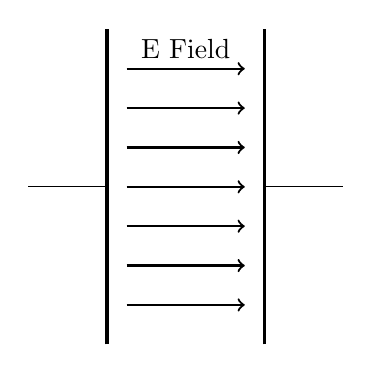
\begin{tikzpicture}
        %% parallel plates
        \draw[very thick] (-1,-2) -- (-1,2);
        \draw[very thick] (+1,-2) -- (+1,2);
        %% wires
        \draw (-1,0) -- (-2,0);
        \draw (+1,0) -- (+2,0);
        %% E field
        \node[anchor=south] at (0,15mm) {E Field};
        \foreach \y in {-15,-10,...,15}
            \draw[thick,->] (-0.75,\y mm) -- ++(0:1.5);
    \end{tikzpicture}
    \end{center}
    Which of the following statements is true?
    \begin{choices}
        \wrongchoice{The field strength decreases.}
        \wrongchoice{The field strength increases.}
      \correctchoice{The potential difference between the plates increases.}
    \end{choices}
\end{questionmult}
}


%% PhysicsBowl 1996
%%----------------------------------------
\element{aapt}{ %% Bowl-D1
\begin{question}{bowl-1996-q21}
    Two isolated conducting spheres ($S_1$ of radius \SI{0.030}{\meter} and initial charge \SI[retain-explicit-plus]{+6.0}{\nano\coulomb} and $S_2$ of radius \SI{0.040}{\meter} and initial charge \SI[retain-explicit-plus]{+2.0}{\nano\coulomb}) are connected by a conducting wire.
    Charge will flow in the wire until:
    \begin{choices}
        \wrongchoice{both spheres are equally charged.}
        \wrongchoice{the net charge is zero.}
        \wrongchoice{the force of repulsion between the two spheres becomes equal.}
        \wrongchoice{both spheres have the same surface charge density.}
      \correctchoice{both spheres are at the same potential.}
    \end{choices}
\end{question}
}

\element{aapt}{ %% Bowl-D1
\begin{question}{bowl-1996-q29}
    Two large parallel plates a distance $d$ apart are charged by connecting them to a battery of potential difference $V$.
    The battery is disconnected, and the plates are slowly moved apart.
    As the distance between plates increases:
    \begin{choices}
        \wrongchoice{the charge on the plates decreases.}
        \wrongchoice{the electric field intensity between the plates increases.}
        \wrongchoice{the electric field intensity between the plates decreases.}
        \wrongchoice{the potential difference between the plates decreases.}
      \correctchoice{the potential difference between the plates increases.}
    \end{choices}
\end{question}
}

\element{aapt}{ %% Bowl-D1
\begin{question}{bowl-1996-q34}
    A point charge $+q$ is placed midway between two point charges $+3q$ and $-q$ separated by a distance $2d$.
    If Coulomb's constant is $k$,
        the magnitude of the force on the charge $+q$ is:
    \begin{multicols}{3}
    \begin{choices}
        \wrongchoice{$2 \dfrac{kq^2}{d^2}$}
      \correctchoice{$4 \dfrac{kq^2}{d^2}$}
        \wrongchoice{$6 \dfrac{kq^2}{d^2}$}
        \wrongchoice{$8 \dfrac{kq^2}{d^2}$}
        \wrongchoice{$10\dfrac{kq^2}{d^2}$}
    \end{choices}
    \end{multicols}
\end{question}
}


%% PhysicsBowl 1995
%%----------------------------------------
\element{aapt}{ %% Bowl-D1
\begin{question}{bowl-1995-q26}
    Two positive point charges repel each other with force \SI{0.36}{\newton} when their separation is \SI{1.5}{\meter}.
    What force do they exert on each other when their separation is \SI{1.0}{\meter}?
    \begin{multicols}{3}
    \begin{choices}
      \correctchoice{\SI{0.81}{\newton}}
        \wrongchoice{\SI{0.54}{\newton}}
        \wrongchoice{\SI{0.36}{\newton}}
        \wrongchoice{\SI{0.24}{\newton}}
        \wrongchoice{\SI{0.25}{\newton}}
    \end{choices}
    \end{multicols}
\end{question}
}


%% PhysicsBowl 1994
%%----------------------------------------
\element{aapt}{ %% Bowl-D1
\begin{questionmult}{bowl-1994-q07}
    A positively charged conductor attracts a second object.
    Which of the following statements could be true?
    \begin{choices}
      \correctchoice{The second object is a conductor with negative net charge.}
      \correctchoice{The second object is a conductor with zero net charge.}
      \correctchoice{The second object is an insulator with zero net charge.}
    \end{choices}
\end{questionmult}
}

\element{aapt}{ %% Bowl-D1
\begin{question}{bowl-1994-q08}
    A point charge of \SI[retain-explicit-plus]{+4.0}{\micro\coulomb} is placed on the negative $x$-axis \SI{0.20}{\meter} to the left of the origin,
        as shown in the accompanying figure.
    \begin{center}
    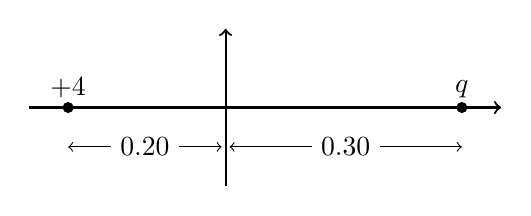
\begin{tikzpicture}
        %% axis
        \draw[thick,->] (-2.5,0) -- (3.5,0);
        \draw[thick,->] (0,-1) -- (0,1);
        %% charges
        \fill (-2,0) circle (2pt) node[anchor=south] {\SI{+4}{\micro\coulomb}};
        \fill (+3,0) circle (2pt) node[anchor=south] {$q$};
        %% distances
        \draw[<->] (-2,-0.5) -- (-0.05,-0.5) node[pos=0.5,anchor=center,fill=white] {\SI{0.20}{\meter}};
        \draw[<->] (+3,-0.5) -- (+0.05,-0.5) node[pos=0.5,anchor=center,fill=white] {\SI{0.30}{\meter}};
    \end{tikzpicture}
    \end{center}
    A second point charge $q$ is placed on the positive $x$-axis \SI{0.30}{\meter} to the right of the origin.
    The net electric field at the origin is zero. 
    What is $q$?
    \begin{multicols}{2}
    \begin{choices}
      \correctchoice{\SI[retain-explicit-plus]{+9.0}{\micro\coulomb}}
        \wrongchoice{\SI[retain-explicit-plus]{+6.0}{\micro\coulomb}}
        \wrongchoice{\SI[retain-explicit-plus]{0.0}{\micro\coulomb}}
        \wrongchoice{\SI[retain-explicit-plus]{-6.0}{\micro\coulomb}}
        \wrongchoice{\SI[retain-explicit-plus]{-9.0}{\micro\coulomb}}
    \end{choices}
    \end{multicols}
\end{question}
}

\element{aapt}{ %% Bowl-D1
\begin{questionmult}{bowl-1994-q21}
    Which of the following statements about solid conductors in electrostatics are true?
    \begin{choices}
      \correctchoice{The electric field inside the conductor is always zero.}
        \wrongchoice{The electric potential inside the conductor is always zero.}
      \correctchoice{Any net charge is on the surface.}
    \end{choices}
\end{questionmult}
}

\element{aapt}{ %% Bowl-D1
\begin{question}{bowl-1994-q39}
    A small object with charge $q$ and weight $mg$ is attached to one end of a string of length $L$.
    The other end is attached to a stationary support.
    The system is placed in a uniform horizontal electric field $E$,
        as shown in the accompanying figure.
    \begin{center}
    \begin{tikzpicture}
        %% ceiling
        \draw (-2,0) -- (2,0);
        \node[anchor=south,pattern=north east lines,minimum width=4cm] at (0,0) {};
        %% pendulum
        \draw[dashed] (0,0) -- (0,-2);
        \draw (0,0) -- (300:3) node[pos=0.66,anchor=south west] {$L$};
        \draw[fill=white!90!black] (300:3) circle (1ex)
            node[anchor=west,xshift=1ex] {$m$};
            %node[anchor=east,xshift=-1ex] {$q$};
        %% angle
        \draw[<->] (0,-1) arc (270:300:1) node[pos=0.5,anchor=north] {$\theta$};
        %% E field
        \node[anchor=west] at (2,-1) {$E$};
        \foreach \y in {-1,-2,-3} \draw[white!50!black,->] (-2,\y) -- (2,\y);
    \end{tikzpicture}
    \end{center}
    In the presence of the field,
        the string makes a constant angle $\theta$ with the vertical.
    What is the sign and magnitude of $q$?
    \begin{choices}
        \wrongchoice{positive, with magnitude $\dfrac{mg}{E}$}
      \correctchoice{positive, with magnitude $\dfrac{mg}{E}\tan\theta$}
        \wrongchoice{negative, with magnitude $\dfrac{mg}{E}$}
        \wrongchoice{negative, with magnitude $\dfrac{mg}{E}\tan\theta$}
        \wrongchoice{negative, with magnitude $\dfrac{E}{mg}\tan\theta$}
    \end{choices}
\end{question}
}


\endinput


